\documentclass[]{article}
\usepackage{lmodern}
\usepackage{amssymb,amsmath}
\usepackage{ifxetex,ifluatex}
\usepackage{fixltx2e} % provides \textsubscript
\ifnum 0\ifxetex 1\fi\ifluatex 1\fi=0 % if pdftex
  \usepackage[T1]{fontenc}
  \usepackage[utf8]{inputenc}
\else % if luatex or xelatex
  \ifxetex
    \usepackage{mathspec}
  \else
    \usepackage{fontspec}
  \fi
  \defaultfontfeatures{Ligatures=TeX,Scale=MatchLowercase}
\fi
% use upquote if available, for straight quotes in verbatim environments
\IfFileExists{upquote.sty}{\usepackage{upquote}}{}
% use microtype if available
\IfFileExists{microtype.sty}{%
\usepackage{microtype}
\UseMicrotypeSet[protrusion]{basicmath} % disable protrusion for tt fonts
}{}
\usepackage[margin=1in]{geometry}
\usepackage{hyperref}
\hypersetup{unicode=true,
            pdftitle={Summary Graphs of NUTR630 Intake},
            pdfauthor={Dave Bridges, Liv Anderson and Rina Hisamatsu},
            pdfborder={0 0 0},
            breaklinks=true}
\urlstyle{same}  % don't use monospace font for urls
\usepackage{color}
\usepackage{fancyvrb}
\newcommand{\VerbBar}{|}
\newcommand{\VERB}{\Verb[commandchars=\\\{\}]}
\DefineVerbatimEnvironment{Highlighting}{Verbatim}{commandchars=\\\{\}}
% Add ',fontsize=\small' for more characters per line
\usepackage{framed}
\definecolor{shadecolor}{RGB}{248,248,248}
\newenvironment{Shaded}{\begin{snugshade}}{\end{snugshade}}
\newcommand{\KeywordTok}[1]{\textcolor[rgb]{0.13,0.29,0.53}{\textbf{{#1}}}}
\newcommand{\DataTypeTok}[1]{\textcolor[rgb]{0.13,0.29,0.53}{{#1}}}
\newcommand{\DecValTok}[1]{\textcolor[rgb]{0.00,0.00,0.81}{{#1}}}
\newcommand{\BaseNTok}[1]{\textcolor[rgb]{0.00,0.00,0.81}{{#1}}}
\newcommand{\FloatTok}[1]{\textcolor[rgb]{0.00,0.00,0.81}{{#1}}}
\newcommand{\ConstantTok}[1]{\textcolor[rgb]{0.00,0.00,0.00}{{#1}}}
\newcommand{\CharTok}[1]{\textcolor[rgb]{0.31,0.60,0.02}{{#1}}}
\newcommand{\SpecialCharTok}[1]{\textcolor[rgb]{0.00,0.00,0.00}{{#1}}}
\newcommand{\StringTok}[1]{\textcolor[rgb]{0.31,0.60,0.02}{{#1}}}
\newcommand{\VerbatimStringTok}[1]{\textcolor[rgb]{0.31,0.60,0.02}{{#1}}}
\newcommand{\SpecialStringTok}[1]{\textcolor[rgb]{0.31,0.60,0.02}{{#1}}}
\newcommand{\ImportTok}[1]{{#1}}
\newcommand{\CommentTok}[1]{\textcolor[rgb]{0.56,0.35,0.01}{\textit{{#1}}}}
\newcommand{\DocumentationTok}[1]{\textcolor[rgb]{0.56,0.35,0.01}{\textbf{\textit{{#1}}}}}
\newcommand{\AnnotationTok}[1]{\textcolor[rgb]{0.56,0.35,0.01}{\textbf{\textit{{#1}}}}}
\newcommand{\CommentVarTok}[1]{\textcolor[rgb]{0.56,0.35,0.01}{\textbf{\textit{{#1}}}}}
\newcommand{\OtherTok}[1]{\textcolor[rgb]{0.56,0.35,0.01}{{#1}}}
\newcommand{\FunctionTok}[1]{\textcolor[rgb]{0.00,0.00,0.00}{{#1}}}
\newcommand{\VariableTok}[1]{\textcolor[rgb]{0.00,0.00,0.00}{{#1}}}
\newcommand{\ControlFlowTok}[1]{\textcolor[rgb]{0.13,0.29,0.53}{\textbf{{#1}}}}
\newcommand{\OperatorTok}[1]{\textcolor[rgb]{0.81,0.36,0.00}{\textbf{{#1}}}}
\newcommand{\BuiltInTok}[1]{{#1}}
\newcommand{\ExtensionTok}[1]{{#1}}
\newcommand{\PreprocessorTok}[1]{\textcolor[rgb]{0.56,0.35,0.01}{\textit{{#1}}}}
\newcommand{\AttributeTok}[1]{\textcolor[rgb]{0.77,0.63,0.00}{{#1}}}
\newcommand{\RegionMarkerTok}[1]{{#1}}
\newcommand{\InformationTok}[1]{\textcolor[rgb]{0.56,0.35,0.01}{\textbf{\textit{{#1}}}}}
\newcommand{\WarningTok}[1]{\textcolor[rgb]{0.56,0.35,0.01}{\textbf{\textit{{#1}}}}}
\newcommand{\AlertTok}[1]{\textcolor[rgb]{0.94,0.16,0.16}{{#1}}}
\newcommand{\ErrorTok}[1]{\textcolor[rgb]{0.64,0.00,0.00}{\textbf{{#1}}}}
\newcommand{\NormalTok}[1]{{#1}}
\usepackage{graphicx,grffile}
\makeatletter
\def\maxwidth{\ifdim\Gin@nat@width>\linewidth\linewidth\else\Gin@nat@width\fi}
\def\maxheight{\ifdim\Gin@nat@height>\textheight\textheight\else\Gin@nat@height\fi}
\makeatother
% Scale images if necessary, so that they will not overflow the page
% margins by default, and it is still possible to overwrite the defaults
% using explicit options in \includegraphics[width, height, ...]{}
\setkeys{Gin}{width=\maxwidth,height=\maxheight,keepaspectratio}
\IfFileExists{parskip.sty}{%
\usepackage{parskip}
}{% else
\setlength{\parindent}{0pt}
\setlength{\parskip}{6pt plus 2pt minus 1pt}
}
\setlength{\emergencystretch}{3em}  % prevent overfull lines
\providecommand{\tightlist}{%
  \setlength{\itemsep}{0pt}\setlength{\parskip}{0pt}}
\setcounter{secnumdepth}{0}
% Redefines (sub)paragraphs to behave more like sections
\ifx\paragraph\undefined\else
\let\oldparagraph\paragraph
\renewcommand{\paragraph}[1]{\oldparagraph{#1}\mbox{}}
\fi
\ifx\subparagraph\undefined\else
\let\oldsubparagraph\subparagraph
\renewcommand{\subparagraph}[1]{\oldsubparagraph{#1}\mbox{}}
\fi

%%% Use protect on footnotes to avoid problems with footnotes in titles
\let\rmarkdownfootnote\footnote%
\def\footnote{\protect\rmarkdownfootnote}

%%% Change title format to be more compact
\usepackage{titling}

% Create subtitle command for use in maketitle
\newcommand{\subtitle}[1]{
  \posttitle{
    \begin{center}\large#1\end{center}
    }
}

\setlength{\droptitle}{-2em}
  \title{Summary Graphs of NUTR630 Intake}
  \pretitle{\vspace{\droptitle}\centering\huge}
  \posttitle{\par}
  \author{Dave Bridges, Liv Anderson and Rina Hisamatsu}
  \preauthor{\centering\large\emph}
  \postauthor{\par}
  \predate{\centering\large\emph}
  \postdate{\par}
  \date{2017-09-03}


\begin{document}
\maketitle

{
\setcounter{tocdepth}{2}
\tableofcontents
}
\begin{Shaded}
\begin{Highlighting}[]
\KeywordTok{library}\NormalTok{(readr)}
\NormalTok{filename <-}\StringTok{ 'https://docs.google.com/spreadsheets/d/e/2PACX-1vQI-b1A4Zd-gx3FuY3lkKbWE0zKUfmAhpFovKOxow5AC1wWQpBsSvOKI0_gtZ4DJu5sj-YM1_1nsKUe/pub?gid=1032535237&single=true&output=csv'}
\NormalTok{data <-}\StringTok{ }\KeywordTok{read_csv}\NormalTok{(filename)}
\end{Highlighting}
\end{Shaded}

These data can be found in
/Users/davebrid/Documents/GitHub/TeachingLectures/Michigan/NUTR630/Evaluation/GradeCraft
Summary/Student Feedback/Onboarding in a file named
\url{https://docs.google.com/spreadsheets/d/e/2PACX-1vQI-b1A4Zd-gx3FuY3lkKbWE0zKUfmAhpFovKOxow5AC1wWQpBsSvOKI0_gtZ4DJu5sj-YM1_1nsKUe/pub?gid=1032535237\&single=true\&output=csv}.
This script was most recently updated on Wed Jan 31 14:10:18 2018.

\section{Analysis}\label{analysis}

\subsection{What Majors}\label{what-majors}

\begin{Shaded}
\begin{Highlighting}[]
\KeywordTok{library}\NormalTok{(forcats)}
\CommentTok{#grouped with most common 4}

\NormalTok{count.majors <-}
\StringTok{  }\NormalTok{data %>%}
\StringTok{  }\KeywordTok{mutate}\NormalTok{(}\StringTok{`}\DataTypeTok{Which discipline most closely matches your undergraduate degree?}\StringTok{`} \NormalTok{=}\StringTok{ }\KeywordTok{fct_lump}\NormalTok{(}\KeywordTok{as.factor}\NormalTok{(data$}\StringTok{`}\DataTypeTok{Which discipline most closely matches your undergraduate degree?}\StringTok{`}\NormalTok{), }\DataTypeTok{n=}\DecValTok{4}\NormalTok{)) %>%}
\StringTok{  }\KeywordTok{group_by}\NormalTok{(}\StringTok{`}\DataTypeTok{Which discipline most closely matches your undergraduate degree?}\StringTok{`}\NormalTok{) %>%}
\StringTok{  }\KeywordTok{count}\NormalTok{() %>%}
\StringTok{  }\KeywordTok{arrange}\NormalTok{(}\KeywordTok{desc}\NormalTok{(n)) %>%}
\StringTok{  }\KeywordTok{ungroup}\NormalTok{() %>%}
\StringTok{  }\KeywordTok{mutate}\NormalTok{(}\StringTok{`}\DataTypeTok{Which discipline most closely matches your undergraduate degree?}\StringTok{`} \NormalTok{=}\StringTok{ }\KeywordTok{fct_recode}\NormalTok{(}\StringTok{`}\DataTypeTok{Which discipline most closely matches your undergraduate degree?}\StringTok{`}\NormalTok{, }\StringTok{"Neuroscience"} \NormalTok{=}\StringTok{ "Psychology-related (Psychology, Neuroscience, etc.)"}\NormalTok{)) }
  
\KeywordTok{par}\NormalTok{(}\DataTypeTok{mar=}\KeywordTok{c}\NormalTok{(}\DecValTok{9}\NormalTok{,}\DecValTok{4}\NormalTok{,}\DecValTok{4}\NormalTok{,}\DecValTok{2}\NormalTok{))}
\KeywordTok{with}\NormalTok{(count.majors, }\KeywordTok{barplot}\NormalTok{(n,}
                          \DataTypeTok{las=}\DecValTok{2}\NormalTok{,}
                          \DataTypeTok{main=}\StringTok{"What is your major?"}\NormalTok{,}
                          \DataTypeTok{col=}\NormalTok{color.scheme,}
                          \DataTypeTok{names.arg=}\StringTok{`}\DataTypeTok{Which discipline most closely matches your undergraduate degree?}\StringTok{`}\NormalTok{))}
\end{Highlighting}
\end{Shaded}

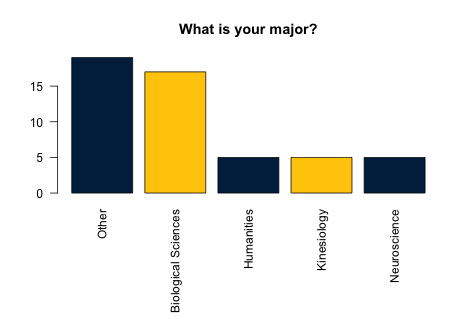
\includegraphics{figures/majors-summary-1.png}

\subsection{What Topics are Students Interested
In?}\label{what-topics-are-students-interested-in}

\begin{Shaded}
\begin{Highlighting}[]
\KeywordTok{library}\NormalTok{(sjPlot)}

\NormalTok{student.interest.data <-}\StringTok{ }
\StringTok{  }\NormalTok{data %>%}
\StringTok{  }\KeywordTok{select}\NormalTok{(}\KeywordTok{starts_with}\NormalTok{(}\StringTok{'Macronutrient'}\NormalTok{),}\KeywordTok{starts_with}\NormalTok{(}\StringTok{"Comprehensive"}\NormalTok{))}


\CommentTok{#manually ensured all columns have same levels}
\NormalTok{mylevels <-}\StringTok{ }\KeywordTok{c}\NormalTok{(}\StringTok{'1'}\NormalTok{,}\StringTok{'2'}\NormalTok{,}\StringTok{'3'}\NormalTok{,}\StringTok{'4'}\NormalTok{,}\StringTok{'5'}\NormalTok{)}
\NormalTok{student.interest.data.levels <-}
\StringTok{  }\NormalTok{student.interest.data}

\NormalTok{student.interest.data.levels$}\StringTok{`}\DataTypeTok{Macronutrient biochemistry is of interest to me.}\StringTok{`} \NormalTok{<-}\StringTok{ }\KeywordTok{factor}\NormalTok{(student.interest.data.levels$}\StringTok{`}\DataTypeTok{Macronutrient biochemistry is of interest to me.}\StringTok{`}\NormalTok{, }\DataTypeTok{levels=}\NormalTok{mylevels)}

\NormalTok{student.interest.data.levels$}\StringTok{`}\DataTypeTok{Macronutrient biochemistry is important for my career interests.}\StringTok{`} \NormalTok{<-}\StringTok{ }\KeywordTok{factor}\NormalTok{(student.interest.data.levels$}\StringTok{`}\DataTypeTok{Macronutrient biochemistry is important for my career interests.}\StringTok{`}\NormalTok{, }\DataTypeTok{levels=}\NormalTok{mylevels)}

\NormalTok{student.interest.data.levels$}\StringTok{`}\DataTypeTok{Comprehensive understanding of the digestive tract is of interest to me.}\StringTok{`} \NormalTok{<-}\StringTok{ }\KeywordTok{factor}\NormalTok{(student.interest.data.levels$}\StringTok{`}\DataTypeTok{Comprehensive understanding of the digestive tract is of interest to me.}\StringTok{`}\NormalTok{, }\DataTypeTok{levels=}\NormalTok{mylevels)}

\NormalTok{student.interest.data.levels$}\StringTok{`}\DataTypeTok{Comprehensive understanding of the digestive tract is important for my career interests.}\StringTok{`} \NormalTok{<-}\StringTok{ }\KeywordTok{factor}\NormalTok{(student.interest.data.levels$}\StringTok{`}\DataTypeTok{Comprehensive understanding of the digestive tract is important for my career interests.}\StringTok{`}\NormalTok{, }\DataTypeTok{levels=}\NormalTok{mylevels)}

\KeywordTok{sjp.likert}\NormalTok{(student.interest.data.levels,}
           \DataTypeTok{sort.frq=}\StringTok{'neg.asc'}\NormalTok{,}
           \DataTypeTok{values=}\StringTok{'hide'}\NormalTok{,}
           \DataTypeTok{show.legend=}\OtherTok{FALSE}\NormalTok{,}
           \DataTypeTok{show.n=}\OtherTok{FALSE}\NormalTok{)}
\end{Highlighting}
\end{Shaded}

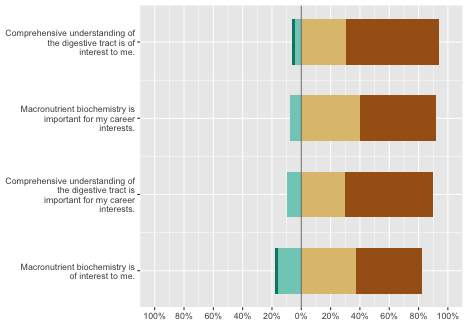
\includegraphics{figures/student-interests-1.png}

\subsection{Learning Assessment}\label{learning-assessment}

\begin{Shaded}
\begin{Highlighting}[]
\NormalTok{student.assessment.data <-}\StringTok{ }
\StringTok{  }\NormalTok{data %>%}
\StringTok{  }\KeywordTok{select}\NormalTok{(}\KeywordTok{starts_with}\NormalTok{(}\StringTok{"What is your level of agreement on the following statements?"}\NormalTok{))}

\KeywordTok{library}\NormalTok{(stringr)}
\KeywordTok{colnames}\NormalTok{(student.assessment.data) <-}\StringTok{ }\KeywordTok{str_sub}\NormalTok{(}\KeywordTok{colnames}\NormalTok{(student.assessment.data), }\DecValTok{63}\NormalTok{, -}\DecValTok{2}\NormalTok{)}

\CommentTok{#manually ensured all columns have same levels}
\NormalTok{mylevels <-}\StringTok{ }\KeywordTok{c}\NormalTok{(}\StringTok{'Strongly Agree'}\NormalTok{,}\StringTok{'Agree'}\NormalTok{,}\StringTok{'Neutral'}\NormalTok{,}\StringTok{'Disagree'}\NormalTok{,}\StringTok{'Strongly Disagree'}\NormalTok{)}

\NormalTok{student.assessment.data$}\StringTok{`}\DataTypeTok{When a difficult assignment is given to me, I feel confident that I can complete it.}\StringTok{`} \NormalTok{<-}\StringTok{ }\KeywordTok{factor}\NormalTok{(student.assessment.data$}\StringTok{`}\DataTypeTok{When a difficult assignment is given to me, I feel confident that I can complete it.}\StringTok{`}\NormalTok{, }\DataTypeTok{levels=}\NormalTok{mylevels)}

\NormalTok{student.assessment.data$}\StringTok{`}\DataTypeTok{When given an assignment to complete, I produce better outcomes with a community of support (i.e., instructor or peer support).}\StringTok{`} \NormalTok{<-}\StringTok{ }\KeywordTok{factor}\NormalTok{(student.assessment.data$}\StringTok{`}\DataTypeTok{When given an assignment to complete, I produce better outcomes with a community of support (i.e., instructor or peer support).}\StringTok{`}\NormalTok{, }\DataTypeTok{levels=}\NormalTok{mylevels)}

\NormalTok{student.assessment.data$}\StringTok{`}\DataTypeTok{I am aware of the skills I develop when I complete different types of assignments.}\StringTok{`} \NormalTok{<-}\StringTok{ }\KeywordTok{factor}\NormalTok{(student.assessment.data$}\StringTok{`}\DataTypeTok{I am aware of the skills I develop when I complete different types of assignments.}\StringTok{`}\NormalTok{, }\DataTypeTok{levels=}\NormalTok{mylevels)}

\NormalTok{student.assessment.data$}\StringTok{`}\DataTypeTok{I am motivated to complete an assignment if I enjoy doing it.}\StringTok{`} \NormalTok{<-}\StringTok{ }\KeywordTok{factor}\NormalTok{(student.assessment.data$}\StringTok{`}\DataTypeTok{I am motivated to complete an assignment if I enjoy doing it.}\StringTok{`}\NormalTok{, }\DataTypeTok{levels=}\NormalTok{mylevels)}

\NormalTok{student.assessment.data$}\StringTok{`}\DataTypeTok{I learn more through completing an assignment that I enjoy.}\StringTok{`} \NormalTok{<-}\StringTok{ }\KeywordTok{factor}\NormalTok{(student.assessment.data$}\StringTok{`}\DataTypeTok{I learn more through completing an assignment that I enjoy.}\StringTok{`}\NormalTok{, }\DataTypeTok{levels=}\NormalTok{mylevels)}

\NormalTok{student.assessment.data$}\StringTok{`}\DataTypeTok{I perform better when completing an assignment that I enjoy (i.e., get a better grade).}\StringTok{`} \NormalTok{<-}\StringTok{ }\KeywordTok{factor}\NormalTok{(student.assessment.data$}\StringTok{`}\DataTypeTok{I perform better when completing an assignment that I enjoy (i.e., get a better grade).}\StringTok{`}\NormalTok{, }\DataTypeTok{levels=}\NormalTok{mylevels)}


\KeywordTok{sjp.likert}\NormalTok{(student.assessment.data,}
           \DataTypeTok{values=}\StringTok{'hide'}\NormalTok{,}
           \DataTypeTok{show.n=}\OtherTok{FALSE}\NormalTok{)}
\end{Highlighting}
\end{Shaded}

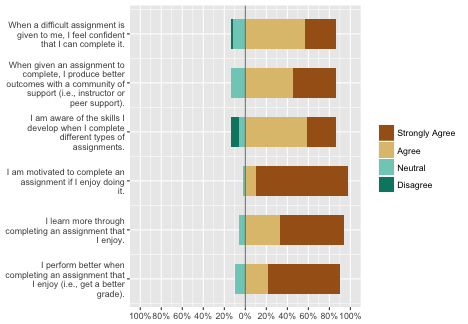
\includegraphics{figures/learning-assessment-1.png}

\section{GradeCraft Familiarity}\label{gradecraft-familiarity}

\begin{Shaded}
\begin{Highlighting}[]
\NormalTok{gradecraft <-}\StringTok{ }
\StringTok{  }\NormalTok{data %>%}
\StringTok{  }\KeywordTok{group_by}\NormalTok{(}\StringTok{`}\DataTypeTok{Are you familiar with GradeCraft?}\StringTok{`}\NormalTok{) %>%}
\StringTok{  }\KeywordTok{count}\NormalTok{()}

\KeywordTok{with}\NormalTok{(gradecraft, }\KeywordTok{barplot}\NormalTok{(n,}
                          \DataTypeTok{las=}\DecValTok{1}\NormalTok{,}
                          \DataTypeTok{ylab=}\StringTok{"Responses"}\NormalTok{,}
                          \DataTypeTok{main=}\StringTok{"Are you familiar with GradeCraft?"}\NormalTok{,}
                          \DataTypeTok{col=}\NormalTok{color.scheme,}
                          \DataTypeTok{names.arg=}\StringTok{`}\DataTypeTok{Are you familiar with GradeCraft?}\StringTok{`}\NormalTok{))}
\end{Highlighting}
\end{Shaded}

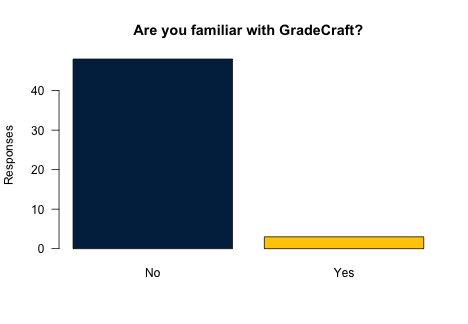
\includegraphics{figures/gradecraft-1.png}

Only 3 out of 51 students were familiar with GradeCraft.

\section{Session Information}\label{session-information}

\begin{Shaded}
\begin{Highlighting}[]
\KeywordTok{sessionInfo}\NormalTok{()}
\end{Highlighting}
\end{Shaded}

\begin{verbatim}
## R version 3.4.2 (2017-09-28)
## Platform: x86_64-apple-darwin15.6.0 (64-bit)
## Running under: macOS High Sierra 10.13.3
## 
## Matrix products: default
## BLAS: /Library/Frameworks/R.framework/Versions/3.4/Resources/lib/libRblas.0.dylib
## LAPACK: /Library/Frameworks/R.framework/Versions/3.4/Resources/lib/libRlapack.dylib
## 
## locale:
## [1] en_US.UTF-8/en_US.UTF-8/en_US.UTF-8/C/en_US.UTF-8/en_US.UTF-8
## 
## attached base packages:
## [1] stats     graphics  grDevices utils     datasets  methods   base     
## 
## other attached packages:
## [1] stringr_1.2.0 sjPlot_2.4.0  bindrcpp_0.2  forcats_0.2.0 readr_1.1.1  
## [6] dplyr_0.7.4   tidyr_0.7.2   knitr_1.17   
## 
## loaded via a namespace (and not attached):
##  [1] nlme_3.1-131       RColorBrewer_1.1-2 rprojroot_1.2     
##  [4] tools_3.4.2        TMB_1.7.12         backports_1.1.1   
##  [7] R6_2.2.2           sjlabelled_1.0.6   DT_0.3            
## [10] lazyeval_0.2.1     colorspace_1.3-2   nnet_7.3-12       
## [13] tidyselect_0.2.3   mnormt_1.5-5       emmeans_1.1       
## [16] curl_3.0           compiler_3.4.2     cli_1.0.0         
## [19] sandwich_2.4-0     effects_4.0-0      scales_0.5.0      
## [22] lmtest_0.9-35      mvtnorm_1.0-7      psych_1.7.8       
## [25] blme_1.0-4         digest_0.6.12      foreign_0.8-69    
## [28] minqa_1.2.4        rmarkdown_1.8      stringdist_0.9.4.6
## [31] pkgconfig_2.0.1    htmltools_0.3.6    lme4_1.1-14       
## [34] pwr_1.2-1          htmlwidgets_1.0    rlang_0.1.4       
## [37] rstudioapi_0.7     shiny_1.0.5        bindr_0.1         
## [40] zoo_1.8-1          magrittr_1.5       modeltools_0.2-21 
## [43] bayesplot_1.4.0    Matrix_1.2-12      Rcpp_0.12.14      
## [46] munsell_0.4.3      abind_1.4-5        prediction_0.2.0  
## [49] stringi_1.1.6      multcomp_1.4-8     yaml_2.1.15       
## [52] merTools_0.3.0     snakecase_0.8.1    carData_3.0-0     
## [55] MASS_7.3-47        plyr_1.8.4         grid_3.4.2        
## [58] parallel_3.4.2     sjmisc_2.6.3       crayon_1.3.4      
## [61] lattice_0.20-35    ggeffects_0.3.1    haven_1.1.0       
## [64] splines_3.4.2      sjstats_0.14.0     hms_0.4.0         
## [67] estimability_1.2   reshape2_1.4.2     codetools_0.2-15  
## [70] stats4_3.4.2       glue_1.2.0         evaluate_0.10.1   
## [73] modelr_0.1.1       httpuv_1.3.5       nloptr_1.0.4      
## [76] gtable_0.2.0       purrr_0.2.4        assertthat_0.2.0  
## [79] ggplot2_2.2.1      mime_0.5           coin_1.2-2        
## [82] xtable_1.8-2       broom_0.4.3        survey_3.32-1     
## [85] coda_0.19-1        survival_2.41-3    tibble_1.3.4      
## [88] arm_1.9-3          glmmTMB_0.2.0      TH.data_1.0-8
\end{verbatim}


\end{document}
